\chapter{Concepts}\label{sec-concepts}

In this section, we will briefly introduce story diagrams and their current features. 
Story diagrams combine
UML activity diagrams and graph transformations by embedding graph replacement rules into the activities.
This allows the activities in Figure \ref{fig:transformationOverview} to be specified formally by graph replacements while preserving the general control flow structure of the example transformation.

In terms of the classification of model transformations proposed by Czarnecki and Helsen~\cite{Czarnecki06}, story diagrams are an endogenous, in-place transformation language.
It has both declarative (pattern matching) and operational elements (specification of control flow):
Its control flow allows a deterministic selection of the graph replacement rules to be applied, with a (non-deterministic) pattern matching in the graph replacement rules.
It can also be used for inter-model transformations to create a new target model from a given source model, as seen in the example given in this paper. 
In order to execute story diagrams, code generation \cite{GBD07} and interpretation \cite{GHS09} are supported.

In the following, we will describe the graph transformations, the so-called story patterns, in Section~\ref{sub:sp}.
Afterwards, we will explain how control flow can be modeled by using elements from activity diagrams in Section~\ref{sub:controlFlow}.

	\section{Expressions} \label{sec:Expressions}
	
	\section{Story Patterns} \label{sec:StoryPatterns}

Story patterns describe graph replacement rules that can be embedded into the activities of a story diagram. They are based on labeled, attributed graphs that are extended by a type model \cite{FNTZ00}. 
The types and references that are specified in the type model are used to type the nodes and edges within the story pattern.
Type models for story diagrams can be created, e.g., by using EMF Ecore \cite{SBP+08}.
In our example, we will use the meta-models shown in Figures~\ref{fig:sourceMetamodel} and~\ref{fig:targetMetamodel} as type models. The type model supports inheritance and polymorphism, i.e., a node of type \fe{Classifier} matches objects of types \fe{Classifier}, \fe{Class}, and \fe{PrimitiveType}.
This allows specifying graph replacement rules for object-oriented models.

In order to provide a concise notation, story patterns apply a short-hand notation depicting left-hand side and right-hand side in one graph. Nodes and edges being created (or deleted) are annotated with \small \verb|<<create>>| \normalsize (or  {\small \verb|<<destroy>>|\normalsize}, respectively). The matching of story patterns in a host graph requires an isomorphic matching of the pattern's left-hand side in the host graph, i.e., two nodes of the pattern may not be matched to the same node in the host graph \cite{FNTZ00,Roz97}. The matching is performed with respect to the types of the type model. The deletion of nodes is applied according to the Single Pushout Approach (SPO, \cite{Roz97}), i.e., dangling edges resulting from the deletion of nodes are deleted as well.

Figure~\ref{fig:SP} shows an example of a story pattern that simply adds a class to the set of classifiers of the source system (cf. Figure~\ref{fig:sourceMetamodel}).

\begin{figure}[htbp]
\begin{center}
  
\includegraphics[width=0.25\textwidth]{figures/StoryPattern}
  \caption{Simple story pattern}
  \label{fig:SP}
\end{center}
\end{figure} 
	
	\section{Story Diagrams} \label{sec:StoryDiagrams}

\subsection*{Old stuff from rejected paper}
Story diagrams are an extension of UML 1.4 activity diagrams \cite{UML} that embed story patterns into the activities.
That allows to model basic control flow structures like branches or loops.
Figure \ref{fig:controlFlow} shows a story diagram that embeds the story pattern of Figure \ref{fig:SP} into one of its activities.
The purpose of the story diagram is to create a new class in the source system if no class with the name given by the parameter \fe{className} already exists. 

\begin{figure}[tbp]
\begin{center}
  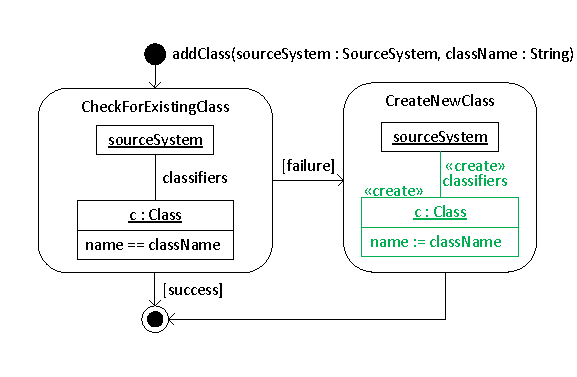
\includegraphics[width=0.7\textwidth]{figures/ControlFlow}
  \caption{Control flow in story diagrams}
  \label{fig:controlFlow}
\end{center}
\end{figure}

In the first activity, the embedded story pattern tries to bind a class with the respective name in the source system. The \fe{sourceSystem} is given as a parameter to the story diagram and can be used as a \emph{bound} node by referring to the name of the parameter. A bound node is signified in the concrete syntax by omitting its type information. Then, the story pattern tries to bind an object of type \fe{Class} to the \emph{unbound} node named \fe{c} such that the attribute condition is fulfilled. 
If this pattern can be matched successfully, i.e., the class already exists, the activity is left via the \fe{[success]} transition and the story diagram terminates.
If no such class can be found, the matching fails and the activity is left via the \fe{[failure]} transition.
Then, the second activity creates the class, links it to the source system, and sets the respective name. 
Additionally, it is possible to add boolean conditions and an \fe{[else]} to the transitions to model more specific conditions.

In general, an initial matching is established by the parameters. This matching is extended by the story patterns in the activities. Then, the matching is propagated to the next activity along the transitions. If a story pattern fails, the current matching is not changed. In subsequent activities, an object previously bound to a node \emph{c} can be referenced using a bound node with name \emph{c}.

The specification of the transformation outlined in Figure~\ref{fig:transformationOverview} can only be accomplished by specifying loops because it requires iterating over all classifiers of the system and all methods of the classes. Loops can be modeled using \emph{forEach activities}.
The story patterns in forEach activities are matched as long as new matchings can be found.
They are visualized by a double border line as depicted in Figure~\ref{fig:forEach}. The transformation formalizes the informal description of Figure~\ref{fig:transformationOverview} using the current features of story diagrams.

\begin{figure}[htb]
\begin{center}
  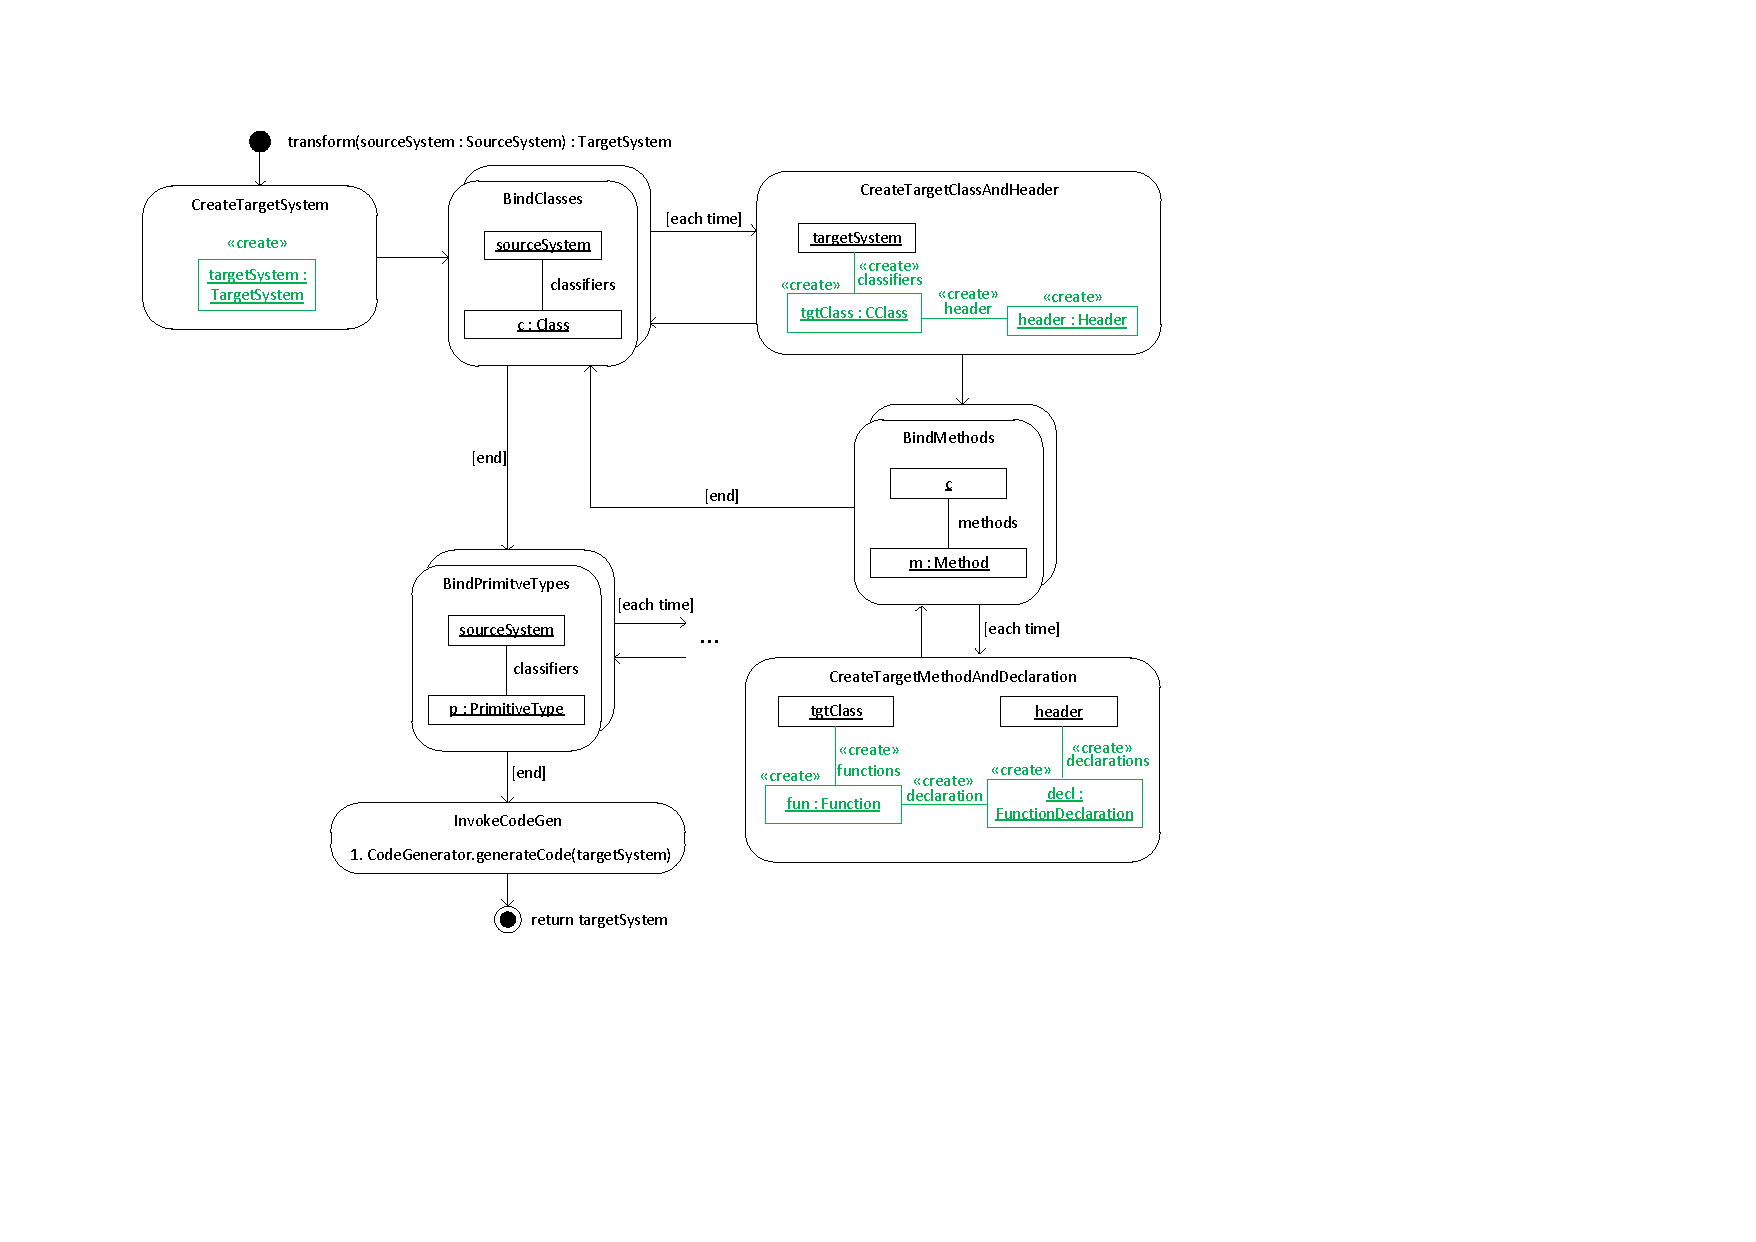
\includegraphics[width=\textwidth]{figures/ForEach}
  \caption{Example of a complex transformation including several forEach activities}
  \label{fig:forEach}
\end{center}
\end{figure}

The story diagram creates a target system in its first activity. Then, all classes of the source system \fe{sourceSystem} are matched. For each match that has been found, the forEach activity is left via the \fe{[each time]} transition. Then, the third activity creates a respective class and its header in the target system. Afterwards, all methods of the class \fe{c} of the source system are matched. Again, the forEach activity is left for each new match using the \fe{[each time]} transition. After all methods have been transformed, the control flow returns to the activity \fe{Bind classes} to bind the next class. It is required that a control flow that has left a forEach activity eventually returns to this activity to obtain a correct story diagram.

After transforming the classes, all primitive types of the source model have to be transformed. We omit the details here due to space limitations. 
Finally, the target system object \fe{targetSystem} is returned by the story diagram as indicated by the annotation \fe{return targetSystem} on the stop node.

Hitherto, story diagrams only support proprietary calls to library functions called collaboration statements. In Figure \ref{fig:forEach}, the activity \fe{InvokeCodeGen} contains such a call to the code generator. The call only is a string expression that does neither allow type checking of the input parameters nor getting a matching of return values, i.e., the return values cannot be used in the story diagram.

\subsection{Applications of Stroy Diagrams (Dietrich)}
2 worlds: with and without methods\ldots

\subsection{General composition of Story Diagrams}
\begin{itemize}
  \item Based on UML 1.5 activity diagrams
  \item Grammar for story diagrams (based on grammar in diploma thesis of Thomas Klein (1999))
\end{itemize}

\subsection{Calls}

\todomvd{Wie sehen Calls (Method/Activity) aus?}